% ---------------------------------------------------------------
% Preamble
% ---------------------------------------------------------------
%\documentclass[a4paper,fleqn,longmktitle]{cas-sc}
\documentclass[a4paper,fleqn]{cas-dc}
%\documentclass[a4paper]{cas-dc}
%\documentclass[a4paper]{cas-sc}
% ---------------------------------------------------------------
% Make margins bigger to fit annotations. TO be removed later
\paperwidth=\dimexpr \paperwidth + 6cm\relax
\oddsidemargin=\dimexpr\oddsidemargin + 3cm\relax
\evensidemargin=\dimexpr\evensidemargin + 3cm\relax
%\marginparwidth=\dimexpr \marginparwidth + 3cm\relax
% -------------------------------------------------------------------- 
% Packages
% --------------------------------------------------------------------
% Figure packages
\usepackage{graphicx,float}
\usepackage{adjustbox}
% Text, input, formatting, and language-related packages
\usepackage[T1]{fontenc}
\usepackage{subcaption}

\usepackage{csvsimple}

\usepackage[bordercolor=gray!20,backgroundcolor=blue!10,linecolor=black,textsize=footnotesize,textwidth=1in]{todonotes}
\setlength{\marginparwidth}{1in}
% \usepackage[utf8]{inputenc}
% \usepackage[nomath]{lmodern}

% Margin and formatting specifications
%\usepackage[authoryear]{natbib}
\usepackage[sort]{natbib}
\setcitestyle{square,numbers}

 %\bibliographystyle{cas-model2-names}

\usepackage{setspace}
\usepackage{subfiles} % Best loaded last in the preamble

% \usepackage[authoryear,longnamesfirst]{natbib}

% Math packages
\usepackage{amsmath, amsthm, amssymb, amsfonts, bm, nccmath, mathdots, mathtools, bigints, ulem}

\usepackage{tikz}
\usepackage{pgfplots}
\usetikzlibrary{shapes.geometric,angles,quotes,calc}

\usepackage[final]{pdfpages}

% --------------------------------------------------------------------
% Packages Configurations
\usepackage{enumitem}
% --------------------------------------------------------------------
% (General) General configurations and fixes
\AtBeginDocument{\setlength{\FullWidth}{\textwidth}}	% Solves els-cas caption positioning issue
\setlength{\parindent}{20pt}
%\doublespacing
% --------------------------------------------------------------------
% Other Definitions
% --------------------------------------------------------------------
\graphicspath{{Figures/}}
% --------------------------------------------------------------------
% Environments
% --------------------------------------------------------------------
% ...

% --------------------------------------------------------------------
% Commands
% --------------------------------------------------------------------

% ==============================================================
% ========================== DOCUMENT ==========================
% ==============================================================
\begin{document} 
%  --------------------------------------------------------------------

% ===================================================
% METADATA
% ===================================================
\title[mode=title]{Parameter estimation}                      
\shorttitle{Parameter estimation}

\shortauthors{A, B, C}

\author[1]{Oliwer Sliczniuk*}[orcid=0000-0003-2593-5956]
\ead{oliwer.sliczniuk@aalto.fi}
\cormark[1]
%\credit{a}

%\author[1]{Pekka Oinas}[orcid=0000-0002-0183-5558]
%\credit{b}

%\author[1]{Francesco Corona}[orcid=0000-0002-3615-1359]
%\credit{c}

\address[1]{Aalto University, School of Chemical Engineering, Espoo, 02150, Finland}
%\address[2]{2}

\cortext[cor1]{Corresponding author}

% ===================================================
% ABSTRACT
% ===================================================
\begin{abstract}
%Given a system of partial differential equations, $F(t,x,\dot{x},p,u)=0$, where $x$ represents state variables, $p$ is the parameters, and $u$ are control variables, the process model is simultaneously solved for both $x_i$ and a set of sensitivity functions, $dx_i/dp_j$, overall times $t$.These sensitivity functions measure the influence of the parameter change on the model's output. As an example, the supercritical extraction process is presented. The impact of mass flow rate, pressure, and inlet temperature on the model's output is discussed. The sensitivity analysis results prove that the considered variables can affect the extraction's yield and be used as control variables in optimization problems. Moreover, the local sensitivity analysis results are analyzed from a phenomenological point of view to enhance understanding of the process model.
%Given a system of partial differential equations, $F(t,x,\dot{x},\Theta,u)=0$, where $x$ represents state variables, $\Theta$ are the parameters, and $u$ are control variables, we describe the supercritical extraction process. The process model describes a partially filled extractor with a fixed bed, which work under constant operating conditions. We assume that the flow is uniform across any cross-section, although the area available for the fluid phase can change along the extractor. We apply the concept of quasi-one-dimensional flow to mimic the modelling of a two-dimensional case.
%In this work, a distributed-parameter model, based on \citet{Reverchon1996} is used to describe a fluid-solid extraction process of caraway oil from caraway seeds with $CO_2$ as a solvent. The model parameters such as partition factor, internal diffusion coefficient, axial diffusion coefficient \textit{and saturation concentration} are obtained from parameter estimation. The parameters are estimated based on four experiments performed at $40^\circ C$/$200$ bar, $50^\circ C$/$200$ bar, $40^\circ C$/$300$ bar and $50^\circ C$/$300$ bar. Given yield data, the model-based parameter estimation uses the maximum likelihood estimation method under assumption of normal error.
We consider a system of partial differential equations, $G(t,x,\dot{x},\Theta,u)=0$, where $x$ denotes the state variables, $\Theta$ represents the parameters, and $u$ is the control variables. Our focus is on the supercritical extraction process, which involves a partially filled extractor with a fixed bed that operates under constant conditions. We assume the flow is uniform across any cross-section, although the area available for the fluid phase can vary along the extractor. To model this two-dimensional case, we use the concept of quasi-one-dimensional flow.
To describe the fluid-solid extraction process of caraway oil from caraway seeds with $CO_2$ as a solvent, we use a distributed-parameter model based on \citet{Reverchon1996}. This model requires parameters such as partition factor, internal diffusion coefficient, axial diffusion coefficient, and an initial state estimate. We estimate these parameters by applying the maximum likelihood estimation method on yield data under the normal error assumption.
The dataset comes from four experiments conducted at different operating conditions: $40^\circ C$/$200$ bar, $50^\circ C$/$200$ bar, $40^\circ C$/$300$ bar, and $50^\circ C$/$300$ bar.

\end{abstract}

\begin{keywords}
Supercritical extraction \sep Parameter estimation \sep Mathematical modeling
\end{keywords}

% ===================================================
% TITLE
% ===================================================
\maketitle

% ===================================================
% Section: Introduction
% ===================================================\section{Introduction}

\section{Introduction}
%\subfile{Sections/introduction}
\subfile{Sections/introduction_imp}

\section{Materials and methods} \label{CH: Materials and methods}

\subsection{Supercritical fluids} \label{CH: Thermodynamic}
%\subfile{Sections/Thermo}
\subfile{Sections/Thermo_imp}

%\clearpage
%\subfile{Sections/Materials_and_methods}

\subsection{Governing equations}
The governing equation for a quasi-one-dimensional compressible flow in Cartesian coordinates can be found in the appendix \ref{CH: Gouverning equations} and in the work of \citet{Anderson1995}.  Quasi-one-dimensional flow is a fluid flow characterized by the assumption that the flow properties remain uniform across any given cross-section of the flow. This assumption is made when there is a variation in the cross-sectional area of the flow channel, such as an irregular shape or partial filling of an extractor. In such cases, the flow is considered to be quasi-one-dimensional because the velocity and other flow properties are assumed to vary only in the direction of flow.

The quasi-one-dimensional compressible Navier-Stokes equations in Cartesian coordinates are given by equations \ref{EQ: CompressibleEuler_1} to \ref{EQ: CompressibleEuler_3}.

{\footnotesize
	\begin{align}
		\label{EQ: CompressibleEuler_1}
		\cfrac{\partial \left( \rho_f A_f \right) }{\partial t} + \cfrac{\partial \left( \rho_f A_f v \right)}{\partial z} &= 0 \\
		\cfrac{\partial \left( \rho_f v A_f \right) }{\partial t} + \cfrac{\partial \left( \rho_f A_f v^2 \right)}{\partial z} &= -A_f \cfrac{\partial P}{\partial z} \label{EQ: CompressibleEuler_2} \\
		\cfrac{\partial \left( \rho_f e A_f \right) }{\partial t} + \cfrac{\partial \left( \rho_f A_f v e\right)}{\partial z} &= -P\cfrac{\left( A_f v \right)}{\partial z} + \cfrac{\partial}{\partial z} \left( \cfrac{\partial T}{\partial z} \right)   
		\label{EQ: CompressibleEuler_3}
	\end{align}  
}

where $\rho_f$ is the density of the fluid, $A_f$ is the function which describe change of the cross-section, $v$ is the velocity, $P$ is the total pressure, $e$ is the internal energy of the fluid, $t$ is time and $z$ is the spacial direction.

Based on governing equations, the small discontinuity (defined as $\delta$) in flow properties, shown in Figure \ref{fig: Discontinuity_slow_flow}, can be analysed. The analysis follows the work of \citet{Schreier1982}.

\begin{figure}[!h]
	\centering
	\resizebox{0.95\columnwidth}{!}{%
		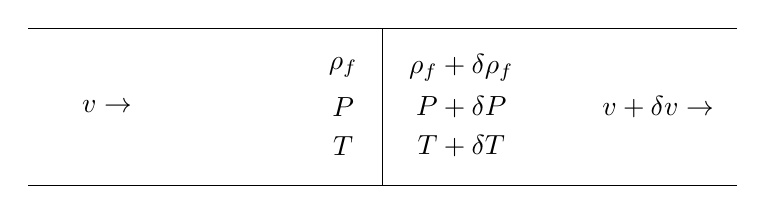
\begin{tikzpicture}[]
			\draw (0,2) -- (9,2);	% Top line
			\draw (0,0) -- (9,0); 	% Bottom line
			\draw (4.5,0) -- (4.5,2); 	% Bottom line
			\node at (4,1.5) {$\rho_f$};
			\node at (5.5,1.5) {$\rho_f+\delta\rho_f$};
			\node at (4,1.0) {$P$};
			\node at (5.5,1.0) {$P+\delta P$};
			\node at (4,0.5) {$T$};
			\node at (5.5,0.5) {$T+\delta T$};
			\node at (1,1.0) {$v \rightarrow$};
			\node at (8,1.0) {$v + \delta v \rightarrow$};
	\end{tikzpicture} }
	\caption{Small discontinuity in one-dimensional flow}
	\label{fig: Discontinuity_slow_flow}
\end{figure} 

The discontinuity is presumed to be at rest relative, and the balance equations become		

{\footnotesize
	\begin{align*}
		&\rho_f \delta v + v \delta \rho_f + \delta \rho_f \delta v = 0 \\
		&\delta P = \delta v \delta \rho_f
	\end{align*}
}

These relations are equally valid if the two regions are separated by a region of finite width rather than a discontinuity. 

{\footnotesize
	\begin{equation*}
		\lim_{\rho_f v \rightarrow 0} \rho_f \delta v + v \delta \rho_f + \delta \rho_f \delta v = 0 / \delta \rho_f \rightarrow \cfrac{d v}{d \rho_f} = - \cfrac{v}{\rho_f}
	\end{equation*}
}

By combining the momentum equation with the above equation, we get

{\footnotesize
	\begin{equation*}
		\cfrac{d v}{d \rho_f} = - \cfrac{d v}{dP} \cfrac{d P}{d \rho_f} = -\cfrac{1}{\rho v} \cfrac{dP}{d\rho_f} = -\cfrac{v}{\rho_f}
	\end{equation*}
}

Suppose the flow is presumed to be isentropic, $dP/d\rho = c^2$, so $v^2=c^2$, where $c$ is the speed of sound. This can be interpreted as a small pressure wave propagating with the speed of sound relative to the flow.

\subsection{Low Mach number expansion}
%\subfile{Sections/Low_mach_number_expansion}
\subfile{Sections/Low_mach_number_expansion_imp}

\subsection{Extraction model} \label{CH: Extraction_model}
\subfile{Sections/Model}

%\newpage
%\section{Bayes theorem} \label{CH: Bayes}
%\subfile{Sections/Bayes_Theorem}
%\clearpage

\subsection{Parameter estimation} \label{CH: Parameter_estimation}
\subfile{Sections/Parameter_estimation}

\subsection{Experimental work}
\subfile{Sections/Experiments}

\section{Results}
\subfile{Sections/Results}

\section{Conclusions}

% ===================================================
% Bibliography
% ===================================================
%% Loading bibliography style file
\clearpage
%\bibliographystyle{model1-num-names}
\bibliographystyle{unsrtnat}
\bibliography{mybibfile}

\clearpage \appendix \label{appendix}
\section{Appendix} 
\subsection{Thermodynamic}
\subfile{Sections/Thermodynamic_details}
\subsection{Governing equations}
\subfile{Sections/Gouverning_equation_derivation}

\subsection{Bayes theorem} \label{CH: Bayes}
\subfile{Sections/Bayes_Theorem}

\subsection{Cardano's Formula} \label{CH: Cardano}
\subfile{Sections/Cardano}

\subsection{Initial and boundary conditions} \label{CH: IC_BC}
\subfile{Sections/IC_BC}

\subsection{Porosity Calculations} \label{CH: Porosity}
\subfile{Sections/Porosity}

\clearpage
\onecolumn
\subsection{Solid density measurement} \label{CH: Solid_Density_Measurment}

\begin{figure*}[!h]
	%\centering 
	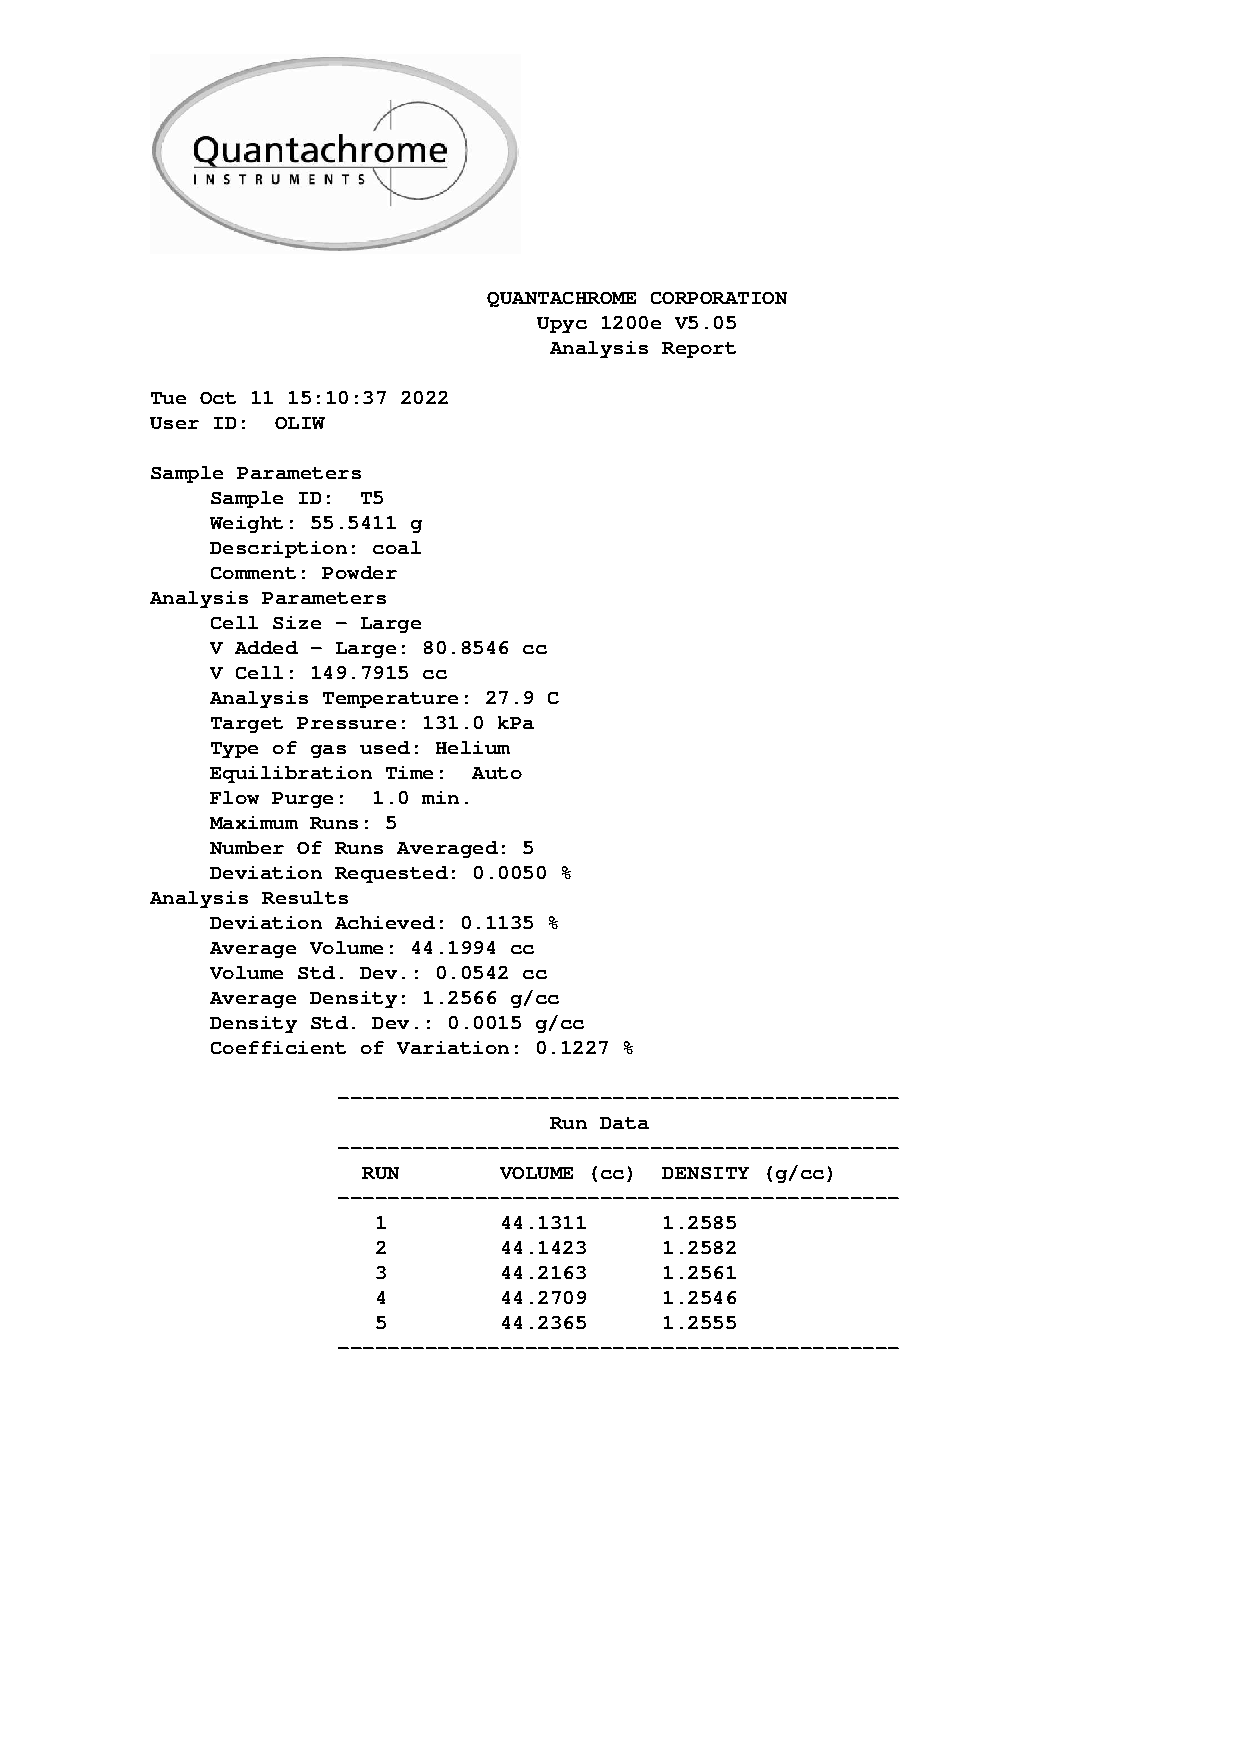
\includegraphics[trim=0cm 6cm 0cm 0cm, clip,height=0.85\textheight]{Sections/ultraReportT5.pdf}
	\caption{The result of solid density measurement}
\end{figure*}

{\footnotesize
	\begin{equation*}
		\rho_s^{ave} = \frac{1.2585+1.2582+1.2561+1.2546+1.2555}{5} = 1.25658 [g/cc]
	\end{equation*}
}

\iffalse
\newpage
\begin{table*}[p]
		\caption{Notation}
		\label{tab::symbols}
		\begin{tabular}{ |c|l|c| } 
			\hline
			Symbol 		& 	Description 							& Unit 						\\ \hline
			$A$			&	cross-section							& $m^2$ 					\\ \hline
			$c$			&	concentration in fluid phase			& $kg ~ m^{-3}$				\\ \hline
			$Cp$		&	specific heat of the fluid				& $J ~ mol^{-1} ~ K^{-1}$ 	\\ \hline
			$Cp_s$		&	specific heat of the solid				& $J ~ mol^{-1} ~ K^{-1}$ 	\\ \hline
			$D_e^M$		&	axial mass diffusion coefficient		& $m^2 ~ s^{-1}$			\\ \hline
			$D_e^T$		&	axial heat diffusion coefficient		& $m^2 ~ s^{-1}$			\\ \hline
			$Di$		&	internal diffusion coefficient			& $m^2 ~ s^{-1}$			\\ \hline
			$dp$		&	particle diameter						& $m$						\\ \hline
			$F(t)$		&	mass flow-rate							& $kg ~ s^{-1}$				\\ \hline
			$km$		&	partition coefficient					& $[-]$						\\ \hline
			$k^T$		&	thermal conductivity					& $W ~ m^{-1} ~ K^{-1}$		\\ \hline
			$l$			&	characteristic dimension				& $m$						\\ \hline
			$L$			&	total length of the bed					& $m$						\\ \hline
			$m$			&	mass of the oil in solid phase			& $kg$						\\ \hline
			$m_0$		&	initial mass of the oil in solid phase	& $kg$						\\ \hline
			$M_{CO_2}$	&	molecular mass of CO2					& $mol ~ kg^{-1}$			\\ \hline
			$Np$		&	number of model parameters and control variables & $[-]$			\\ \hline
			$N_{\theta}$&	number of model parameters				& $[-]$						\\ \hline
			$Nu$		&	number of control variables				& $[-]$						\\ \hline
			$Nz$		&	number of grid points in z-direction	& $[-]$						\\ \hline
			$p$			&	vector of model parameters and control variables	& $[-]$			\\ \hline
			$P(t)$		&	pressure								& $bar$						\\ \hline
			$Pe$		&	Peclet's number							& $[-]$						\\ \hline
			$q$			&	concentration in solid phase			& $kg ~ m^{-3}$				\\ \hline
			$R$			&	gas constant							& $J ~ K^{-1} ~ mol^{-1}$	\\ \hline
			$Re$		&	Reynolds number							& $[-]$						\\ \hline
			$t$			&	time									& $s$						\\ \hline
			$T$			&	temperature								& $K$						\\ \hline
			$T_0$		&	initial temperature						& $K$						\\ \hline
			$V$			&	volume of the extractor					& $m^3$						\\ \hline
			$y$			&	yield	 								& $[-]$						\\ \hline
			$z$			&	length									& $m$						\\ \hline
			$Z$			&	compressibility	factor					& $[-]$						\\ \hline
			$\epsilon$	&	void fraction							& $[-]$						\\ \hline
			$\rho$		&	density of the fluid					& $kg ~ m^{-3}$				\\ \hline
			$\rho_s$	&	solid density							& $kg ~ m^{-3}$				\\ \hline
			$\mu$		&	shape coefficient						& $[-]$						\\ \hline
			$\theta$	&	vector of model parameters				& $[-]$						\\ \hline
			$\eta$		&	viscosity								& $cP$						\\ \hline				
						& 											&							\\ \hline			
		 	Subscript	& 											&							\\ \hline
			$0$			&	initial conditions						& $[-]$						\\ \hline
			$^*$		&	equilibrium conditions					& $[-]$						\\ \hline							
		\end{tabular}
\end{table*}
\fi
\end{document}